\chapter{Calculus}
% From Gilbert Strang book chapter 13
$$ f(x,y) \quad x \in \mathbb{R}, y \in \mathbb{R} $$


Example
We have a function of two dimensional space $z = f(x,y)$.
Example:

\begin{itemize}
    \item Traveling wave $f(x,t) = \cos(x-t)$
    \item $f(x, y) = 3x + y + 1$
    \item $f: \mathbb{R}^n \rightarrow \mathbb{R} $
\end{itemize}

Up to now, we used linear Algebra to solve this problem.
Now we want to use calculus.

$$
x = \begin{pmatrix}
x_1 \\
x_2
\end{pmatrix} \quad A =
\begin{pmatrix}
    a_{11} & a_{12} \\
    a_{21} & a_{22}
\end{pmatrix} \quad b = \begin{pmatrix}
    b_1 \\
    b_2
    \end{pmatrix} \quad \min_{x} \|Ax-b\|^2_2 = \min_x f(x)
$$

$$
\min_{x_1, x_2} f(x) = \min_{x_1, x_2} \left( (a_{11}x_1 + a_{12}x_2 - b_1)^2 + (a_{21}x_1 + a_{22}x_2 - b_2)^2 \right)
$$

We compute the derivative of $f(x)$ first fixing $x_2$ and then $x_1$.

$$ f'(x_1) = 2(a_{11}x_1 + a_{12}x_2 - b_1)a_{11} + 2(a_{21}x_1 + a_{22}x_2 - b_2)a_{21} $$ 
$$ f'(x_2) = 2(a_{11}x_1 + a_{12}x_2 - b_1)a_{12} + 2(a_{21}x_1 + a_{22}x_2 - b_2)a_{22} $$

Since we want to find the minimum, we set the derivative to zero $f'(x_1) = 0$ and $f'(x_2) = 0$.

$$
\begin{aligned}
    f'(x_1) &= 0 \Leftrightarrow a_{11}^2x_1 + a_{11}a_{12}x_2 - a_{11}b_1 + a_{21}a_{11}x_1 + a_{21}a_{12}x_2 - a_{21}b_2 = 0 \\
    &= a_{11}^2x_1 + a_{11}a_{12}x_2 + a_{21}a_{11}x_1 + a_{21}a_{12}x_2 = a_{11}b_1 + a_{21}b_2 \\
    &= (a_{11}^2 + a_{21}a_{11})x_1 + (a_{11}a_{12} + a_{21}a_{12})x_2 = a_{11}b_1 + a_{21}b_2 \\
\end{aligned}
$$
$$
\begin{aligned}
    f'(x_2) &= 0 \Leftrightarrow a_{11}a_{12}x_1 + a_{12}^2x_2 - a_{12}b_1 + a_{21}a_{12}x_1 + a_{22}a_{12}x_2 - a_{22}b_2 = 0 \\
    &= a_{11}a_{12}x_1 + a_{12}^2x_2 + a_{21}a_{12}x_1 + a_{22}a_{12}x_2 = a_{12}b_1 + a_{22}b_2 \\
    &= (a_{11}a_{12} + a_{21}a_{12})x_1 + (a_{12}^2 + a_{22}a_{12})x_2 = a_{12}b_1 + a_{22}b_2 \\
\end{aligned}
$$

$$
\begin{cases}
    (a_{11}^2 + a_{21}a_{11})x_1 + (a_{11}a_{12} + a_{21}a_{12})x_2 = a_{11}b_1 + a_{21}b_2 \\
    (a_{11}a_{12} + a_{21}a_{12})x_1 + (a_{12}^2 + a_{22}a_{12})x_2 = a_{12}b_1 + a_{22}b_2 \\
\end{cases}
\Leftrightarrow
A^TAx = A^Tb
$$
\section{Partial Derivatives}

Partial derivatives are a fundamental concept in calculus, particularly in the field of multivariable calculus. They represent the rate of change of a function with respect to one of its variables, while keeping the other variables constant.

Let \( f: \mathbb{R}^n \rightarrow \mathbb{R} \) be a function of \( n \) variables, say \( f(x_1, x_2, \ldots, x_n) \). The partial derivative of \( f \) with respect to its \( i \)-th variable \( x_i \) is denoted as \( \frac{\partial f}{\partial x_i} \) and is defined as:

\[
\frac{\partial f}{\partial x_i}(x_1, x_2, \ldots, x_n) = \lim_{h \rightarrow 0} \frac{f(x_1, \ldots, x_i + h, \ldots, x_n) - f(x_1, \ldots, x_i, \ldots, x_n)}{h}
\]

if this limit exists. In other words, the partial derivative of \( f \) with respect to \( x_i \) at a point is the slope of the tangent line to the curve you get by fixing every variable except \( x_i \) and graphing \( f \) as a function of \( x_i \) alone.

\subsection{Geometric Interpretation}
In the context of a function of two variables, \( f(x, y) \), the partial derivatives \( \frac{\partial f}{\partial x} \) and \( \frac{\partial f}{\partial y} \) represent the slope of the tangent plane to the surface defined by \( f \) in the direction of the \( x \)-axis and \( y \)-axis respectively.

\subsection{Higher Order Partial Derivatives}
If the partial derivatives of a function are themselves differentiable, we can take their partial derivatives. These are known as higher-order partial derivatives. For instance, the second-order partial derivative of \( f \) with respect to \( x_i \) and then \( x_j \) is denoted as \( \frac{\partial^2 f}{\partial x_j \partial x_i} \).

\subsection{Hessian Matrix}
The matrix that collects all the second-order partial derivatives of a scalar-valued function is called the Hessian matrix. For a function \( f: \mathbb{R}^n \rightarrow \mathbb{R} \), the Hessian matrix is defined as:
$$ H = \begin{pmatrix}
\frac{\partial^2 f}{\partial x_1^2} & \frac{\partial^2 f}{\partial x_1 \partial x_2} & \cdots & \frac{\partial^2 f}{\partial x_1 \partial x_n} \\
\frac{\partial^2 f}{\partial x_2 \partial x_1} & \frac{\partial^2 f}{\partial x_2^2} & \cdots & \frac{\partial^2 f}{\partial x_2 \partial x_n} \\
\vdots & \vdots & \ddots & \vdots \\
\frac{\partial^2 f}{\partial x_n \partial x_1} & \frac{\partial^2 f}{\partial x_n \partial x_2} & \cdots & \frac{\partial^2 f}{\partial x_n^2}
\end{pmatrix} $$
The Hessian matrix is symmetric if all the second-order partial derivatives are continuous.

Following the example, the related Hessian matrix is:
$$
\begin{aligned}
\frac{\partial^2 f}{\partial x_1^2} = \frac{\partial}{\partial x_1} &\left( 2(a_{11}x_1 + a_{12}x_2 - b_1)a_{11} + 2(a_{21}x_1 + a_{22}x_2 - b_2)a_{21} \right) = 2(a_{11}^2 + a_{21}^2) \\
\frac{\partial^2 f}{\partial x_2 \partial x_1} = \frac{\partial}{\partial x_2} &\left( 2(a_{11}x_1 + a_{12}x_2 - b_1)a_{11} + 2(a_{21}x_1 + a_{22}x_2 - b_2)a_{21} \right) = 2(a_{12}a_{11} + a_{22}a_{21}) \\
\frac{\partial^2 f}{\partial x_1 \partial x_2} = \frac{\partial}{\partial x_1} &\left( 2(a_{11}x_1 + a_{12}x_2 - b_1)a_{12} + 2(a_{21}x_1 + a_{22}x_2 - b_2)a_{22} \right) = 2(a_{12}a_{11} + a_{22}a_{21}) \\
\frac{\partial^2 f}{\partial x_2^2} = \frac{\partial}{\partial x_2} &\left( 2(a_{11}x_1 + a_{12}x_2 - b_1)a_{12} + 2(a_{21}x_1 + a_{22}x_2 - b_2)a_{22} \right) = 2(a_{12}^2 + a_{22}^2) \\
\end{aligned}
$$
$$ H = \begin{pmatrix}
2(a_{11}^2 + a_{21}^2) & 2(a_{12}a_{11} + a_{22}a_{21}) \\
2(a_{12}a_{11} + a_{22}a_{21}) & 2(a_{12}^2 + a_{22}^2)
\end{pmatrix} = 2A^TA
$$

\subsection{Gradient}
The gradient is a vector-valued function, which takes a scalar-valued function of multiple variables as input, and returns a vector where each entry is a partial derivative of the input function. The gradient of a function \( f: \mathbb{R}^n \rightarrow \mathbb{R} \) is denoted as \( \nabla f \) and is defined as:
$$ \nabla f = \begin{pmatrix}
\frac{\partial f}{\partial x_1} \\
\frac{\partial f}{\partial x_2} \\
\vdots \\
\frac{\partial f}{\partial x_n}
\end{pmatrix} $$

\subsection{Tangent line}
The tangent line to a curve at a given point is the straight line that "just touches" the curve at that point.
Leibniz defined it as the line through a pair of infinitely close points on the curve
More precisely, a straight line is said to be a tangent of a curve \( y = f(x) \) at a
point \( x = c \) on the curve if the line passes through the point \( (c, f(c)) \) on
the curve and has slope \( f'(c) \), where \( f' \) denotes the derivative of \( f \).
A similar definition applies to space curves and curves in n-dimensional Euclidean space.

% https://www.geogebra.org/3d
\pgfplotsset{compat=newest}

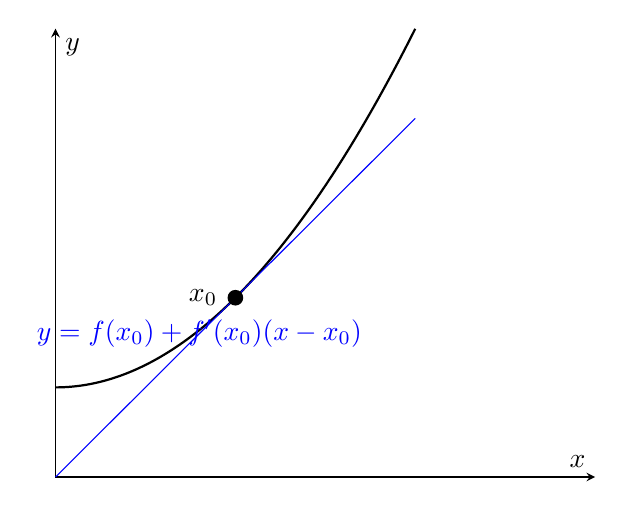
\begin{tikzpicture}
    \begin{axis}[
        axis lines = middle,
        xlabel = \( x \),
        ylabel = \( y \),
        xtick=\empty,
        ytick=\empty,
        clip=false,
        ymin=0,
        ymax=5,
        xmin=0,
        xmax=3
    ]
    
    % Curve equation
    \addplot [domain=0:2, samples=100, smooth, thick] {x^2 + 1};
    
    % Tangent line equation at x0
    \pgfmathsetmacro{\xZero}{1}
    \pgfmathsetmacro{\yZero}{(\xZero)^2 + 1}
    \pgfmathsetmacro{\derivative}{2*\xZero}
    \addplot [domain=0:2, samples=2, smooth, color=blue] {\derivative*(x - \xZero) + \yZero} node[pos=0.4]{$y = f(x_0) + f'(x_0)(x-x_0)$};
    
    % Point of tangency
    \node[label={180:{\( x_0 \)}},circle,fill,inner sep=2pt] at (axis cs:\xZero,\yZero) {};
    
    \end{axis}
    \end{tikzpicture}

$x_0$ is a stationary point of the function $f(x)$ if $f'(x_0) = 0$.
If we use the taylor polynomial
$$f(x) = f(x_0) + f'(x_0)(x-x_0) + \frac{f''(x_0)}{2}(x-x_0)^2 + \ldots$$

We have that
$$f(x) \approx f(x_0) + \frac{f''(x_0)}{2}(x-x_0)^2 + \ldots \quad f'(x_0) = 0 $$

\subsection{Tangent plane}

$$ f(x, y) = x^2y^2 + xy + y $$
$$ \frac{\partial f}{\partial x} = 2xy^2 + y \quad \frac{\partial f}{\partial y} = 2x^2y + x + 1 $$
$$ z = x_0^2y_0^2 + x_0y_0 + y_0 + \frac{\partial f}{\partial x}(x_0, y_0)(x-x_0) + \frac{\partial f}{\partial y}(x_0, y_0)(y-y_0) $$
$$ z = x_0^2y_0^2 + x_0y_0 + y_0 + (2x_0y_0^2 + y_0)(x-x_0) + (2x_0^2y_0 + x_0 + 1)(y-y_0) $$
$z$ is the tangent plane to $(x_0, y_0)$.

\subsection{The normal vector to a surface}
The normal vector to a surface at a point is a vector that is perpendicular to the tangent plane to that surface at the point.
The normal vector to a surface at a point \( (x_0, y_0) \) is given by:
$$ \vec{n} = \nabla f(x_0, y_0) = \begin{pmatrix}
\frac{\partial f}{\partial x}(x_0, y_0) \\
\frac{\partial f}{\partial y}(x_0, y_0) \\
\end{pmatrix} $$
where \( f \) is a function of two variables.


\section{Differentials}
The differential of a function \( f: \mathbb{R}^n \rightarrow \mathbb{R} \) is defined as:
$$ df = \frac{\partial f}{\partial x_1} dx_1 + \frac{\partial f}{\partial x_2} dx_2 + \cdots + \frac{\partial f}{\partial x_n} dx_n $$
where \( dx_i \) is the differential of the \( i \)-th variable \( x_i \).

\section{Artificial Neural Networks}

\subsection{Activation functions}
Activation functions are used to introduce non-linearity in neural networks.
Sigmoid, ReLU, tanh, Leaky ReLU, ELU, Softmax, Swish, etc.

Sigmoid:
$$\sigma(x) = \frac{1}{1+e^{-x}}, \quad \sigma'(x) = \sigma(x)(1-\sigma(x))$$
$$\tanh(x) = \frac{e^x - e^{-x}}{e^x + e^{-x}}, \quad \tanh'(x) = 1 - \tanh^2(x)$$


% \begin{tikzpicture}
% \begin{axis}[
%     axis lines = middle,
%     xlabel = \( x \),
%     ylabel = \( y \),
%     xtick=\empty,
%     ytick=\empty,
%     clip=false,
%     ymin=0,
%     ymax=1,
%     xmin=-5,
%     xmax=5
% ]
% \plot[domain=-5:5, samples=100, smooth, thick] {1/(1+exp(-x))};
% \end{axis}
% \end{tikzpicture}

\section{Direction derivative}
The directional derivative of a multivariate differentiable function along a given vector \( \vec{v} \) at a given point \( \vec{x} \) intuitively represents the instantaneous rate of change of the function, moving through \( \vec{x} \), in the direction of \( \vec{v} \). It therefore generalizes the notion of a partial derivative, in which the rate of change is taken along the direction of one of the coordinate axes, all other coordinates being constant.

The directional derivative of a function \( f: \mathbb{R}^n \rightarrow \mathbb{R} \) at a point \( \vec{x} \) in the direction \( \vec{v} \) is defined as:
$$ D_{\vec{v}} f(\vec{x}) = \lim_{h \rightarrow 0} \frac{f(\vec{x} + h\vec{v}) - f(\vec{x})}{h} $$
if this limit exists. In other words, the directional derivative of \( f \) at \( \vec{x} \) in the direction \( \vec{v} \) is the slope of the tangent line to the curve you get by fixing every variable except \( \vec{v} \) and graphing \( f \) as a function of \( \vec{v} \) alone.

\section{Positive definite matrix}
In linear algebra, a symmetric \( n \times n \) real matrix \( M \) is said to be positive definite if the scalar \( z^TMz \) is strictly positive for every non-zero column vector \( z \) of \( n \) real numbers. Here \( z^T \) denotes the transpose of \( z \).

Let be \( A \in \mathbb{R}^{n \times n} \) a symmetric matrix. \( A \) is positive definite if and only if all its eigenvalues are positive.


